% !TeX root = ../main.tex

% Edit this title for each week's entry.
\section{Week 8 - Financial Accounting}

\topic{Introduction to Financial Accounting}

\heading{Purpose of Accounting}
\begin{itemize}
    \item \b{Measure} business activity
    \item \b{Financial reporting}:
    \begin{itemize}
        \item Internal: decision makers
        \item External: investors; government (tax authorities, regulators)
    \end{itemize}
\end{itemize}

\heading{Types of Accounting}
\begin{center}
\begin{tabular}{p{0.2\linewidth}p{0.34\linewidth}p{0.34\linewidth}}
    \toprule
    & \rb{Managerial} (internal use) & \rb{Financial} (external use) \\
    \midrule
    Users & Internal decision makers / managers, controllers & Investors / creditors, government \\
    Presentation & Company specific; \dbb{future oriented} (assumptions) & Must conform to standards / regulations (\dbb{GAAP}) \\
    \bottomrule
\end{tabular}
\end{center}

\heading{How to Organize a Business}
\begin{itemize}
    \item \rb{Proprietorship}: owned by one person
    \item \rb{Partnership}: owned by two or more partners
    \item \rb{Corporation}: a separate legal entity owned by its shareholders
\end{itemize}

\begin{definition}[GAAP]
    \rb{Generally Accepted Accounting Principles}: the rules that govern
    accounting (accountants follow professional guidelines).
    \begin{itemize}
        \item \b{Primary objective}: to provide information useful for making investment (including lending) decisions
        \item \b{Useful information} is \dbb{relevant}, \dbb{reliable}, and \dbb{comparable}
    \end{itemize}
\end{definition}

\heading{Accounting Principles}
\begin{enumerate}
    \item \rb{Entity concept}: the business is accounted for separately from its owners
    \item \rb{Relevance characteristic}: report information that helps users make decisions
    \item \rb{Reliability / objectivity principle}: records are based on verifiable, unbiased evidence
    \item \rb{Cost principle}: assets are recorded at their actual (historical) cost
    \item \rb{Going-concern concept}: assume the business will keep operating into the foreseeable future
    \item \rb{Stable monetary unit concept}: assume the dollar's purchasing power is stable (ignore inflation)
\end{enumerate}

\begin{definition}[Financial Statements]
    Financial information about a business entity, prepared in a
    systematic report format that decision makers can use: the
    \rb{income statement}, \rb{balance sheet}, \rb{statement of cash flows},
    and \rb{statement of retained earnings}.
\end{definition}

\heading{Balance Sheet and Income Statement}
\begin{itemize}
    \item \b{Balance sheet}: a ``\dbb{snapshot in time}''
    \item \b{Income statement}: the performance of the business \dbb{over a period of time}
\end{itemize}
\begin{center}
    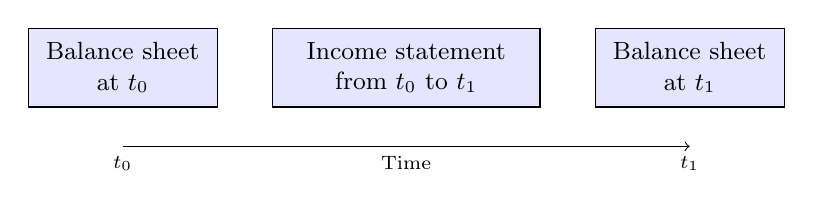
\begin{tikzpicture}[box/.style={draw,fill=blue!10,align=center,minimum height=1cm,font=\small}]
        \node[box,minimum width=2.4cm] (b0) at (0,0) {Balance sheet\\at $t_0$};
        \node[box,minimum width=3.4cm] (is) at (3.6,0) {Income statement\\from $t_0$ to $t_1$};
        \node[box,minimum width=2.4cm] (b1) at (7.2,0) {Balance sheet\\at $t_1$};
        \draw[->] (0,-1) node[below] {\scriptsize $t_0$} -- (7.2,-1) node[below] {\scriptsize $t_1$};
        \node[below] at (3.6,-1) {\scriptsize Time};
    \end{tikzpicture}
\end{center}

\begin{definition}[The Accounting Equation]
    \[\boxed{\text{Assets} = \text{Liabilities} + \text{Owners' (Shareholders') Equity}}\]
\end{definition}

\heading{The Five Basic Accounts}
The \rb{account} is accounting's main summary device: the record of
changes.
\begin{center}
\begin{tabular}{ll}
    \toprule
    \b{Balance sheet} (\dbb{permanent} accounts) & \b{Income statement} (\dbb{temporary} accounts) \\
    \midrule
    \rb{Assets}: short term and long term & \rb{Revenues} \\
    \rb{Liabilities}: short term and long term & \rb{Expenses} \\
    \rb{Equity}: paid-in and retained earnings & \\
    \bottomrule
\end{tabular}
\end{center}

\begin{itemize}
    \item \rb{Assets}: economic resources that benefit the business now and in the future
    \begin{itemize}
        \item Current: cash, accounts receivable, inventory, notes receivable, prepaid expenses
        \item Long term: land, buildings, equipment, furniture and fixtures
    \end{itemize}
    \item \rb{Liabilities}: the debts of the company. Bank loan, notes payable, accounts payable, accrued liabilities (expenses incurred but not paid), long-term liabilities (bonds and mortgages)
    \item \rb{Shareholders' (owners') equity}: the owners' claims to the assets of a corporation
    \begin{itemize}
        \item Contributed capital
        \item Retained earnings: increases by revenues $-$ expenses
    \end{itemize}
\end{itemize}

\heading{Components of Retained Earnings}
\begin{center}
    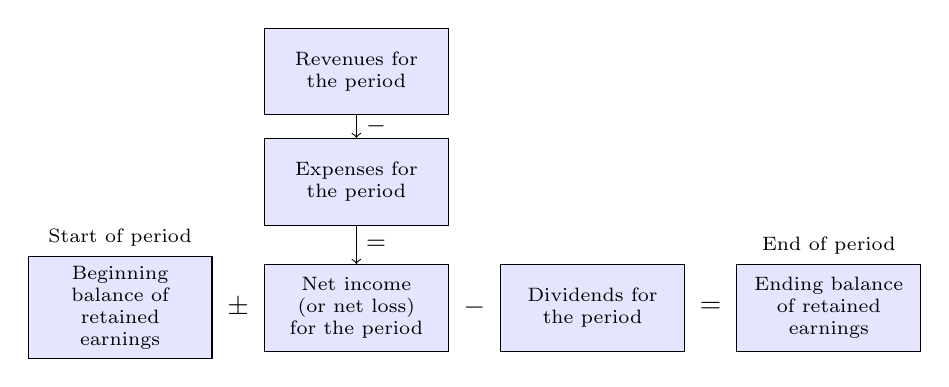
\begin{tikzpicture}[box/.style={draw,fill=blue!10,align=center,minimum height=1.1cm,text width=2.1cm,font=\scriptsize}]
        \node[box] (rev) at (3,3) {Revenues for the period};
        \node[box] (exp) at (3,1.6) {Expenses for the period};
        \node[box] (beg) at (0,0) {Beginning balance of retained earnings};
        \node[box] (ni) at (3,0) {Net income (or net loss) for the period};
        \node[box] (div) at (6,0) {Dividends for the period};
        \node[box] (end) at (9,0) {Ending balance of retained earnings};
        \draw[->] (rev) -- node[right,font=\small] {$-$} (exp);
        \draw[->] (exp) -- node[right,font=\small] {$=$} (ni);
        \node at (1.5,0) {$\pm$};
        \node at (4.5,0) {$-$};
        \node at (7.5,0) {$=$};
        \node[above,font=\scriptsize] at (beg.north) {Start of period};
        \node[above,font=\scriptsize] at (end.north) {End of period};
    \end{tikzpicture}
\end{center}
\[\boxed{\text{RE}_{\text{end}} = \text{RE}_{\text{begin}} + (\text{Revenues} - \text{Expenses}) - \text{Dividends}}\]

\begin{definition}[Transaction]
    Any event that has a \dbb{financial impact} on the business.
    Transactions can be measured reliably, provide objective information,
    and must have a \$ amount assigned to the event.
\end{definition}

\heading{The Basis: Accrual or Cash}
\begin{itemize}
    \item \rb{Accrual accounting}: ``transactions are recorded \dbb{when they occur}, not when the cash is actually exchanged''
    \begin{itemize}
        \item You may pay tax on money you have not yet received, but you can also claim expenses you have not paid yet
        \item In both cases, there is evidence that something has happened
    \end{itemize}
    \item \rb{Cash basis accounting}: transactions are recognized when cash changes hands
    \item Accrual is used in almost all businesses; cash basis is useful for small cash-based businesses
\end{itemize}

\begin{remark}
    Don't confuse the cash \emph{basis} with ``cash-flow''!
\end{remark}

\begin{definition}[Double-Entry Accounting]
    Traces back to 1494 (Luca Pacioli, the ``father of accounting''). Uses
    \rb{debits} and \rb{credits} to record the \dbb{dual effects} of each
    business transaction. Each account is drawn as a \rb{T-account}:
    \begin{center}
        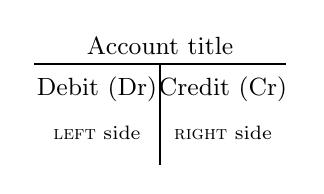
\begin{tikzpicture}[scale=0.8]
            \draw[thick] (-2,0) -- (2,0);
            \draw[thick] (0,0) -- (0,-1.6);
            \node[above] at (0,0) {\small Account title};
            \node at (-1,-0.4) {\small Debit (Dr)};
            \node at (1,-0.4) {\small Credit (Cr)};
            \node at (-1,-1.1) {\scriptsize \textsc{left} side};
            \node at (1,-1.1) {\scriptsize \textsc{right} side};
        \end{tikzpicture}
    \end{center}
\end{definition}

\heading{Rules of Debit and Credit}
\begin{center}
\begin{tabular}{lcc}
    \toprule
    Account & Debit (left) & Credit (right) \\
    \midrule
    Assets & $+$ & $-$ \\
    Liabilities & $-$ & $+$ \\
    Shareholders' equity & $-$ & $+$ \\
    \midrule
    Expenses (decrease equity) & $+$ & $-$ \\
    Revenues (increase equity) & $-$ & $+$ \\
    \bottomrule
\end{tabular}
\end{center}
\db{Assets sit on the \dbb{left} of the accounting equation, so they increase with a debit; liabilities and equity sit on the \dbb{right}, so they increase with a credit.}

\begin{example}[Owner Investment]
    The owner of a business invests \$50,000 cash in the business.
    \\\db{Cash (asset) goes up: \dbb{debit} Cash \$50,000. Equity goes up: \dbb{credit} Shareholders' equity \$50,000. Both sides of the accounting equation rise by \$50,000, so it still balances.}
\end{example}

\heading{Income Statement Accounts: Revenues and Expenses}
Income statement accounts are \dbb{temporary}: they are ``closed out'' (into
retained earnings) at the end of each reporting period.
\begin{itemize}
    \item \rb{Revenues}: sales associated with the business. They increase shareholders' equity, so they are recorded as \dbb{credits}
    \item \rb{Expenses}: costs incurred by the business. They decrease shareholders' equity, so they are recorded as \dbb{debits}
\end{itemize}

\heading{Summary}
\begin{enumerate}
    \item Accounting measures business activity for internal and external users; financial accounting follows GAAP
    \item Main statements: the \b{balance sheet} (snapshot) and \b{income statement} (over a period)
    \item Five basic accounts: assets, liabilities, equity (permanent); revenues, expenses (temporary)
    \item Assets $=$ Liabilities $+$ Equity
\end{enumerate}

\topic{Example: Tara Inc.\ (Service Industry)}

\begin{example}[Tara Inc.]
    Record the following January 2021 transactions for Tara Inc.\ (TI), a
    new engineering services company, and build its balance sheet and
    income statement.
    \begin{center}
    \small
    \begin{tabular}{clp{0.6\linewidth}r}
        \toprule
        \# & Date & Item & Amount \\
        \midrule
        1 & 1-Jan & TI received \$50k cash from shareholders and issued common shares & 50,000 \\
        2 & 1-Jan & TI paid \$40k cash for land & 40,000 \\
        3 & 1-Jan & TI borrowed \$10k from a bank (5-year loan, 8\% interest, payable yearly) & 10,000 \\
        4 & 1-Jan & TI purchased office supplies for \$3700 on accounts payable & 3,700 \\
        5 & 31-Jan & TI performed engineering services for clients and received \$7k cash & 12,000 \\
        6 & 31-Jan & TI performed services for King Inc.\ on account and invoiced King for \$3k & 3,000 \\
        7 & 31-Jan & TI paid \$2700 for expenses: office rent \$1100, salary \$1200, utilities \$400 & 2,700 \\
        8 & 31-Jan & TI paid \$1900 on the account payable & 1,900 \\
        9 & 31-Jan & TI collected \$1000 from King & 1,000 \\
        10 & 31-Jan & TI sold a portion of its land for \$22k (no gain or loss) & 22,000 \\
        11 & 31-Jan & TI paid its shareholders dividends of \$2100 & 2,100 \\
        12 & 31-Jan & Interest on loan & 67 \\
        13 & 31-Jan & Taxes for January (20\%) & \\
        \bottomrule
    \end{tabular}
    \end{center}
    \db{Start from an all-zero balance sheet (new business). For each transaction, find the two (or more) accounts affected, then debit/credit by the rules above. Total debits always equal total credits.}
    \begin{center}
    \small
    \begin{tabular}{clrlr}
        \toprule
        \# & Debit (Dr) & & Credit (Cr) & \\
        \midrule
        1 & Cash & 50,000 & Common shares & 50,000 \\
        2 & Land & 40,000 & Cash & 40,000 \\
        3 & Cash & 10,000 & Long-term debt & 10,000 \\
        4 & Office supplies & 3,700 & Accounts payable & 3,700 \\
        5 & Cash & 7,000 & Revenue & 12,000 \\
          & Accounts receivable & 5,000 & & \\
        6 & Accounts receivable & 3,000 & Revenue & 3,000 \\
        7 & Office rent & 1,100 & Cash & 2,700 \\
          & Salary expense & 1,200 & & \\
          & Utilities & 400 & & \\
        8 & Accounts payable & 1,900 & Cash & 1,900 \\
        9 & Cash & 1,000 & Accounts receivable & 1,000 \\
        10 & Cash & 22,000 & Land & 22,000 \\
        11 & Dividends paid & 2,100 & Cash & 2,100 \\
        12 & Interest expense & 67 & Interest payable & 67 \\
        13 & Taxes & 2,447 & Taxes payable & 2,447 \\
        \bottomrule
    \end{tabular}
    \end{center}
    \db{Notes on the trickier entries:}
    \begin{itemize}
        \item \db{\#4, \#6: bought/sold \dbb{on account}, so no cash moves yet (accrual basis). The supplies are an asset; the service is revenue now, collected later as a receivable}
        \item \db{\#5: the work was worth \$12,000 but only \$7,000 was paid in cash, so the other \$5,000 is a receivable}
        \item \db{\#8, \#9: paying a payable or collecting a receivable is \dbb{not} an expense or revenue (that was recorded already); only cash changes}
        \item \db{\#11: dividends are \dbb{not} an expense; they reduce retained earnings directly}
        \item \db{\#12: one month of interest, accrued but not yet paid: $10{,}000 \times 8\%/12 = \$66.67 \approx \$67$}
        \item \db{\#13: tax on income before taxes: $0.20 \times 12{,}233 = \$2{,}446.60 \approx \$2{,}447$, owed but not yet paid}
    \end{itemize}
    \db{Final income statement (January 2021) and balance sheet (31-Jan-2021):}
    \begin{center}
    \small
    \begin{minipage}[t]{0.42\linewidth}\centering
        \begin{tabular}[t]{lr}
            \toprule
            \multicolumn{2}{c}{\b{Income Statement}} \\
            \midrule
            Revenue & 15,000 \\
            \quad Salary expense & 1,200 \\
            \quad Office rent & 1,100 \\
            \quad Utilities & 400 \\
            Total operating expenses & 2,700 \\
            \midrule
            Operating income & 12,300 \\
            \quad Interest expense & 67 \\
            Income before taxes & 12,233 \\
            \quad Provision for taxes & 2,447 \\
            \midrule
            \b{Net income} & \b{9,786} \\
            \quad Dividends & 2,100 \\
            Addition to equity & 7,686 \\
            \bottomrule
        \end{tabular}
    \end{minipage}
    \hfill
    \begin{minipage}[t]{0.55\linewidth}\centering
        \begin{tabular}[t]{lr|lr}
            \toprule
            \multicolumn{4}{c}{\b{Balance Sheet}} \\
            \midrule
            Cash & 43,300 & Acc.\ payable & 1,800 \\
            Acc.\ receivable & 7,000 & Interest payable & 67 \\
            Office supplies & 3,700 & Taxes payable & 2,447 \\
            \b{Current} & 54,000 & \b{Current} & 4,314 \\
            Land & 18,000 & Long-term debt & 10,000 \\
            & & \b{Liabilities} & 14,314 \\
            & & Common shares & 50,000 \\
            & & Retained earnings & 7,686 \\
            & & \b{Equity} & 57,686 \\
            \midrule
            \b{Total assets} & \b{72,000} & \b{Total L + E} & \b{72,000} \\
            \bottomrule
        \end{tabular}
    \end{minipage}
    \end{center}
    \db{Check: Cash $= 50 - 40 + 10 + 7 - 2.7 - 1.9 + 1 + 22 - 2.1 = \$43.3$k. The sheet balances: $72{,}000 = 14{,}314 + 57{,}686$. Retained earnings started at 0, so $\text{RE} = 0 + 9{,}786 - 2{,}100 = 7{,}686$.}
\end{example}

\heading{Key Points}
\begin{itemize}
    \item For every credit there is a debit, and vice versa
    \item To increase a \b{left-hand} account (assets, expenses) we \dbb{debit}
    \item To increase a \b{right-hand} account (liabilities, equity, revenues) we \dbb{credit}
    \item This example started from a zero balance sheet (new business). Next month's starting point would be this month's \dbb{ending} balance sheet
\end{itemize}

\topic{Financial Ratios}

\heading{Financial Ratio Classification}
\begin{enumerate}
    \item Ability to pay current liabilities (\rb{liquidity ratios})
    \item Ability to sell inventory and collect receivables (\rb{efficiency ratios})
    \item Ability to pay long-term debt (\rb{leverage ratios})
    \item \rb{Profitability ratios}
    \item Analysis of shares as an investment (\rb{performance ratios})
\end{enumerate}

\begin{example}[Meben Furniture Ltd.]
    All ratios below use Meben's statements.
    \begin{center}
    \small
    \begin{minipage}[t]{0.44\linewidth}\centering
        \begin{tabular}[t]{lr}
            \toprule
            \multicolumn{2}{c}{\b{Income Statement (2019)}} \\
            \midrule
            Net sales & \$858,000 \\
            Cost of goods sold & 513,000 \\
            Gross margin & \$345,000 \\
            Total operating expenses & 244,000 \\
            Income from operations & \$101,000 \\
            Interest revenue & (4,000) \\
            Interest expense & 24,000 \\
            Income before taxes & \$81,000 \\
            Income taxes & 33,000 \\
            \b{Net income} & \b{\$48,000} \\
            \bottomrule
        \end{tabular}
    \end{minipage}
    \hfill
    \begin{minipage}[t]{0.53\linewidth}\centering
        \begin{tabular}[t]{lrr}
            \toprule
            \b{Balance Sheet} & 2019 & 2018 \\
            \midrule
            Cash & \$29,000 & \$32,000 \\
            Receivables, net & 114,000 & 85,000 \\
            Inventories & 113,000 & 111,000 \\
            Prepaid expenses & 6,000 & 8,000 \\
            \b{Total current assets} & \$262,000 & \$236,000 \\
            Long-term investments & 18,000 & 9,000 \\
            Plant and equipment, net & 507,000 & 399,000 \\
            \b{Total assets} & \$787,000 & \$644,000 \\
            \midrule
            Notes payable & \$42,000 & \$27,000 \\
            Accounts payable & 73,000 & 68,000 \\
            Accrued liabilities & 27,000 & 31,000 \\
            \b{Total current liabilities} & 142,000 & 126,000 \\
            Long-term debt & 289,000 & 198,000 \\
            \b{Total liabilities} & \$431,000 & \$324,000 \\
            \midrule
            Common shares & \$186,000 & \$186,000 \\
            Retained earnings & 170,000 & 134,000 \\
            \b{Total equity} & 356,000 & 320,000 \\
            \b{Total L + E} & \$787,000 & \$644,000 \\
            \bottomrule
        \end{tabular}
    \end{minipage}
    \end{center}
    Meben has 10,000 shares outstanding, a share price of \$60, and paid a
    dividend of \$1.20 per share.
\end{example}

\heading{1. Liquidity Ratios}
\begin{definition}[Current Ratio]
    The company's ability to pay current liabilities with current assets:
    \[\boxed{\text{Current ratio} = \frac{\text{Current assets}}{\text{Current liabilities}}}\]
\end{definition}
\[\text{2019: } \frac{262{,}000}{142{,}000} = \db{1.85}, \qquad \text{2018: } \frac{236{,}000}{126{,}000} = \db{1.87} \qquad (\text{industry average } 1.50)\]

\begin{definition}[Acid-Test (Quick) Ratio]
    The company's ability to pay all current liabilities \dbb{if they come
    due immediately} (excludes inventory and prepaid expenses, which can't
    be turned into cash quickly):
    \[\boxed{\text{Acid-test ratio} = \frac{\text{Cash} + \text{Short-term investments} + \text{Net current receivables}}{\text{Current liabilities}}}\]
\end{definition}
\[\text{2019: } \frac{29{,}000 + 114{,}000}{142{,}000} = \db{1.01}, \qquad \text{2018: } \frac{32{,}000 + 85{,}000}{126{,}000} = \db{0.93} \qquad (\text{industry } 0.40)\]
\db{Meben is comfortably above the industry on both liquidity ratios.}

\heading{2. Efficiency Ratios}
\begin{definition}[Inventory Turnover]
    The number of times the average level of inventory is sold during a
    year. A \dbb{high} number means inventory sells quickly:
    \[\boxed{\text{Inventory turnover} = \frac{\text{COGS}}{\text{Average inventory}}, \qquad \text{Days' inventory} = \frac{\text{Average inventory}}{\text{COGS}/365}}\]
    Days' inventory is the inverse of inventory turnover, times the number
    of days in the period.
\end{definition}
\[\text{Turnover} = \frac{513{,}000}{(113{,}000 + 111{,}000)/2} = \db{4.6}, \qquad \text{Days' inventory} = \frac{112{,}000}{513{,}000/365} = \db{80 \text{ days}}\]
\db{Industry average turnover is 3.4, i.e.\ $365/3.4 \approx 107$ days (the slide uses 3.5 to get 104 days). Meben sells its inventory faster.}

\begin{definition}[Accounts Receivable Turnover]
    A company's ability to collect cash from credit customers:
    \[\boxed{\text{A/R turnover} = \frac{\text{Net credit sales}}{\text{Average net A/R}}, \qquad \text{Days' receivables} = \frac{\text{Average A/R}}{\text{Sales}/365}}\]
    If credit sales aren't reported separately, use total sales.
\end{definition}
\[\text{Turnover} = \frac{858{,}000}{(114{,}000 + 85{,}000)/2} = \db{8.6 \text{ times}}, \qquad \text{Days' receivables} = \frac{99{,}500}{858{,}000/365} = \db{42 \text{ days}}\]
\db{Industry average is 51 times, i.e.\ $365/51 = 7$ days. Meben takes much longer than the industry to collect from customers.}

\heading{3. Leverage Ratios}
\begin{definition}[Debt Ratio]
    The proportion of assets financed with debt:
    \[\boxed{\text{Debt ratio} = \frac{\text{Total liabilities}}{\text{Total assets}}}\]
\end{definition}
\[\text{2019: } \frac{431{,}000}{787{,}000} = \db{0.55}, \qquad \text{2018: } \frac{324{,}000}{644{,}000} = \db{0.50} \qquad (\text{industry } 0.64)\]

\begin{definition}[Times-Interest-Earned]
    The number of times operating income can cover interest expense:
    \[\boxed{\text{Times-interest-earned} = \frac{\text{Income from operations}}{\text{Interest expense}} = \frac{\text{EBIT}}{\text{Interest expense}}}\]
\end{definition}
\[\text{2019: } \frac{101{,}000}{24{,}000} = \db{4.21} \qquad (\text{industry } 2.80)\]
\db{Meben uses less debt than the industry and covers its interest more easily.}

\heading{4. Profitability Ratios}
\begin{definition}[Profit Margin]
    The percentage of each sales dollar earned as net income:
    \[\boxed{\text{Profit margin} = \frac{\text{Net income}}{\text{Net sales}}}\]
\end{definition}
\[\text{2019: } \frac{48{,}000}{858{,}000} = \db{0.056} \qquad (\text{industry } 0.008)\]

\begin{definition}[Return on Assets (ROA)]
    How profitably the company uses its assets. There are a few different
    formulas; the key is to be \dbb{consistent}:
    \[\boxed{\text{ROA} = \frac{\text{Net income}}{\text{Assets}} \quad\text{or}\quad \text{ROA} = \frac{\text{Net income} + \text{Interest}(1 - \text{Tax rate})}{\text{Assets}}}\]
    The second version adds back the after-tax interest, so it measures the
    return on assets regardless of how they were financed.
\end{definition}
\db{Using 2019 total assets, and tax rate $= 33{,}000/81{,}000 = 40.7\%$:}
\[\text{ROA} = \frac{48{,}000}{787{,}000} = \db{0.061}, \qquad \text{ROA} = \frac{48{,}000 + 24{,}000(1 - 0.407)}{787{,}000} = \db{0.079} \qquad (\text{industry } 0.078)\]

\begin{definition}[Return on Equity (ROE)]
    How much the company has earned on funds invested by shareholders
    (directly and through retained earnings):
    \[\boxed{\text{ROE} = \frac{\text{Net income}}{\text{Equity}}}\]
\end{definition}
\[\text{2019: } \frac{48{,}000}{356{,}000} = \db{0.135} \qquad (\text{industry } 0.121)\]

\begin{definition}[Earnings per Share (EPS)]
    The profits of a company on a per-share basis. Investors pay particular
    attention to EPS:
    \[\boxed{\text{EPS} = \frac{\text{Net income}}{\text{Total shares outstanding}}}\]
\end{definition}
\[\text{EPS} = \frac{48{,}000}{10{,}000} = \db{\$4.80}\]

\heading{5. Performance Ratios (Shares as an Investment)}
\begin{definition}[Price to Earnings (P/E) Ratio]
    Relates a company's share price to its earnings per share:
    \[\boxed{\text{P/E} = \frac{\text{Share price}}{\text{EPS}}}\]
    \begin{itemize}
        \item A high P/E could mean the stock is \dbb{overvalued}, or that investors expect \dbb{high future growth}
        \item Companies with no earnings (or losing money) have no P/E
        \item Leverage affects P/E, so be careful when comparing companies
    \end{itemize}
\end{definition}
\[\text{P/E} = \frac{\$60}{\$4.80} = \db{12.5}\]

\begin{definition}[Dividend Yield]
    How much a company pays out in dividends each year relative to its
    share price:
    \[\boxed{\text{Dividend yield} = \frac{\text{Dividend per share}}{\text{Price per share}}}\]
    Mature, stable companies are the most likely to pay dividends; high-growth
    companies typically do not.
\end{definition}
\[\text{Dividend yield} = \frac{\$1.20}{\$60} = \db{0.02}\]

\begin{definition}[Market Capitalization]
    Not a ratio: the total dollar market value of a company's outstanding
    shares:
    \[\boxed{\text{Market cap} = \text{Price per share} \times \text{Shares outstanding}}\]
    Companies are typically divided into \b{large-cap} (\$10 billion or
    more), \b{mid-cap} (\$2--10 billion) and \b{small-cap} (\$300 million
    to \$2 billion).
\end{definition}
\[\text{Market cap} = \$60 \times 10{,}000 = \db{\$600{,}000}\]

\heading{Summary}
\begin{center}
\begin{tabular}{ll}
    \toprule
    Category & Ratios \\
    \midrule
    Liquidity & Current ratio, acid-test ratio \\
    Efficiency & Inventory turnover / days' inventory, A/R turnover / days' receivables \\
    Leverage & Debt ratio, times-interest-earned \\
    Profitability & Profit margin, ROA, ROE, EPS \\
    Performance & P/E, dividend yield, market capitalization \\
    \bottomrule
\end{tabular}
\end{center}
